\section{Approach Overview}
\label{overview:sec}

\subsection{Important Concepts}
\label{concepts:sec}

\begin{Definition}[Program Dependence Graph]
  by Program Dependency Graph (PDG)
  (Look at Definition 3.1 in Flexeme paper)
\end{Definition}

\begin{Definition}[Multi-version Program Dependence Graph]
(Look at Definition 3.2 in Flexeme paper)
\end{Definition}

\begin{figure*}[t]
	\centering
        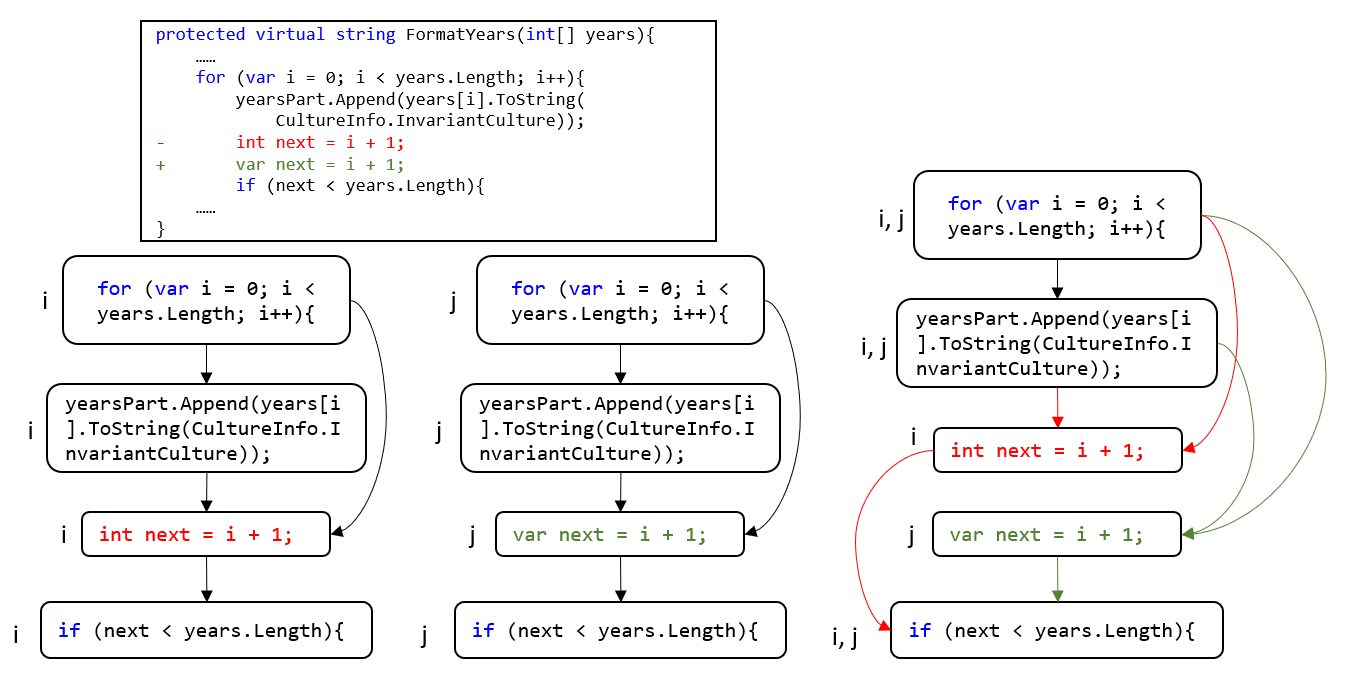
\includegraphics[width=5.3in]{figures/multi-version-graph.png}
        \vspace{-6pt}
	\caption{FIXME: Multi-Version PDG}
	\label{fig:pdg}
\end{figure*}

\begin{Definition}[Changed/Un-changed Statements]
Label 1,2: unchanged, label 1: deleted,...
\end{Definition}


\begin{Definition}[Context]
The context of a changed node is ...
\end{Definition}

\subsection{Architecture Overview}
